\section{Resultados}
\label{sec:resultados}

En esta sección se presentan los resultados analíticos cuantitativos de validación de los componentes, las simulaciones computacionales y las mediciones experimentales obtenidas en el prototipo físico.

\subsection{Validación Analítica Cuantitativa del Enlace}
\label{subsec:calculos_analiticos}

A partir de los parámetros de los componentes seleccionados y descritos en la Tabla~\ref{tab:componentes}, se dedujeron cuantitativamente los modelos de ganancia, potencia y transferencia de datos.

\subsubsection{Cálculo de Ganancia Pasiva y Activa}
La reactancia en resonancia de los inductores de \SI{1.0}{\milli\henry} a la frecuencia portadora $f_0 = \SI{125.04}{\kilo\hertz}$ es:
\begin{equation}
    X_{L0} = \omega_0 L_2 = 2\pi (125040)(\num{1e-3}) = \SI{785.65}{\ohm}
\end{equation}
El factor de calidad no cargado del inductor con resistencia serie parásita $R_{\text{ESR}} = \SI{10}{\ohm}$ resulta:
\begin{equation}
    Q_0 = \frac{X_{L0}}{R_{\text{ESR}}} = \frac{785.65}{10} \approx 78.56 \quad (\SI{37.90}{\deci\bel})
\end{equation}
La resistencia equivalente paralela del tanque a la resonancia alcanza $R_p \approx Q_0^2 R_{\text{ESR}} \approx \SI{61.72}{\kilo\ohm}$. No obstante, al conectarse a la entrada del preamplificador inversor MCP6002 ($R_{\text{in1}} = \SI{10}{\kilo\ohm}$), la impedancia equivalente bajo carga disminuye a:
\begin{equation}
    R_{p,\text{eff}} = R_p \parallel R_{\text{in1}} = \frac{61.72 \times 10}{61.72 + 10} \approx \SI{8.60}{\kilo\ohm}
\end{equation}
reduciendo el factor de calidad cargado efectivo a:
\begin{equation}
    Q_{\text{eff}} = \frac{R_{p,\text{eff}}}{X_{L0}} = \frac{\num{8.60e3}}{785.65} \approx 10.95 \quad (\SI{20.79}{\deci\bel})
\end{equation}

En cuanto a la etapa activa, la ganancia teórica en baja frecuencia (DC) de las dos etapas inversoras en cascada es:
\begin{equation}
    A_{v1,\text{DC}} = -\frac{\SI{68}{\kilo\ohm}}{\SI{10}{\kilo\ohm}} = -6.8, \quad A_{v2,\text{DC}} = -\frac{\SI{47}{\kilo\ohm}}{\SI{10}{\kilo\ohm}} = -4.7
\end{equation}
\begin{equation}
    A_{v,\text{DC}} = A_{v1,\text{DC}} \times A_{v2,\text{DC}} = 31.96\text{ V/V} \quad (\SI{30.09}{\deci\bel})
\end{equation}

Sin embargo, dado que el circuito integrado MCP6002 posee un producto ganancia-ancho de banda finito $\text{GBW} = \SI{1.0}{\mega\hertz}$, el polo de corte a \SI{-3}{\deci\bel} para cada etapa viene determinado por la ganancia de ruido en lazo cerrado ($1 + R_f / R_{\text{in}}$):
\begin{equation}
    f_{c1} = \frac{\text{GBW}}{1 + |A_{v1}|} = \frac{\SI{1000}{\kilo\hertz}}{1 + 6.8} \approx \SI{128.21}{\kilo\hertz}
\end{equation}
\begin{equation}
    f_{c2} = \frac{\text{GBW}}{1 + |A_{v2}|} = \frac{\SI{1000}{\kilo\hertz}}{1 + 4.7} \approx \SI{175.44}{\kilo\hertz}
\end{equation}
Evaluando la respuesta armónica a la portadora de $f_0 = \SI{125}{\kilo\hertz}$:
\begin{equation}
    |A_{v1}(f_0)| = \frac{6.8}{\sqrt{1 + (125 / 128.21)^2}} \approx 4.87
\end{equation}
\begin{equation}
    |A_{v2}(f_0)| = \frac{4.7}{\sqrt{1 + (125 / 175.44)^2}} \approx 3.83
\end{equation}
La ganancia activa real a \SI{125}{\kilo\hertz} es $A_{v,\text{activa}} \approx 4.87 \times 3.83 \approx 18.63\text{ V/V}$ (\SI{25.41}{\deci\bel}). Por tanto, la ganancia global del sistema receptor bajo condiciones reales de carga y ancho de banda resulta:
\begin{equation}
    A_{\text{total,real}} = Q_{\text{eff}} \times A_{v,\text{activa}} \approx 10.95 \times 18.63 \approx 204.09\text{ V/V} \quad (\SI{46.20}{\deci\bel})
\end{equation}

\begin{table}[htbp]
\caption{Resumen del Análisis Cuantitativo de Ganancias}
\label{tab:ganancias}
\centering
\begin{tabular}{lccc}
\toprule
\textbf{Etapa de Ganancia} & \textbf{Teórica Ideal} & \textbf{Efectiva / Real} & \textbf{Atenuación / Causa} \\
\midrule
Tanque RX ($Q$) & $78.56\text{ V/V}$ & $10.95\text{ V/V}$ & Carga $R_{\text{in1}} = \SI{10}{\kilo\ohm}$ \\
Etapa 1 MCP6002 & $6.80\text{ V/V}$ & $4.87\text{ V/V}$ & Límite GBW ($f_{c1} = \SI{128.2}{\kilo\hertz}$) \\
Etapa 2 MCP6002 & $4.70\text{ V/V}$ & $3.83\text{ V/V}$ & Límite GBW ($f_{c2} = \SI{175.4}{\kilo\hertz}$) \\
Ganancia Activa & $31.96\text{ V/V}$ & $18.63\text{ V/V}$ & Limitación dinámica Op-Amp \\
\textbf{Ganancia Global} & $\mathbf{2510\text{ V/V}}$ & $\mathbf{204.09\text{ V/V}}$ & Efecto acoplado carga + GBW \\
\bottomrule
\end{tabular}
\end{table}

\subsubsection{Balance y Estimación de Potencia}
En la etapa transmisora (alimentación $V_{CC} = \SI{5.0}{\volt}$), el driver TC4427A excita el tanque serie con una onda cuadrada simétrica. La primera componente armónica de Fourier es:
\begin{equation}
    V_{1,\text{pk}} = \frac{2 V_{CC}}{\pi} = \frac{2 (5.0)}{\pi} \approx \SI{3.183}{\volt} \implies V_{1,\text{rms}} = \frac{3.183}{\sqrt{2}} \approx \SI{2.251}{\volt}
\end{equation}
La impedancia total en resonancia serie es $Z_{\text{TX}} = R_{\text{limit}} + R_{\text{ESR}} + R_{DS(\text{on})} = 150 + 10 + 3.5 = \SI{163.50}{\ohm}$, lo que establece una corriente fundamental eficaz de:
\begin{equation}
    I_{\text{rms}} = \frac{V_{1,\text{rms}}}{Z_{\text{TX}}} = \frac{\SI{2.251}{\volt}}{\SI{163.50}{\ohm}} = \SI{13.77}{\milli\ampere} \quad (I_{\text{pk}} = \SI{19.47}{\milli\ampere})
\end{equation}
La disipación activa en el tanque serie se distribuye en:
\begin{itemize}
    \item Resistor de límite ($R_{\text{limit}} = \SI{150}{\ohm}$): $P_{\text{limit}} = I_{\text{rms}}^2 R_{\text{limit}} = \SI{28.43}{\milli\watt}$.
    \item Resistencia de bobina ($R_{\text{ESR}} = \SI{10}{\ohm}$): $P_{\text{ESR}} = I_{\text{rms}}^2 R_{\text{ESR}} = \SI{1.90}{\milli\watt}$.
    \item Resistencia interna MOSFET driver: $P_{\text{driver}} = I_{\text{rms}}^2 R_{DS(\text{on})} = \SI{0.66}{\milli\watt}$.
\end{itemize}
La potencia reactiva almacenada en el campo magnético del inductor es:
\begin{equation}
    Q_{\text{mag}} = I_{\text{rms}}^2 X_{L0} = (\num{13.77e-3})^2 \times 785.65 \approx \SI{148.89}{\milli\volt\ampere\text{ reactivo}}
\end{equation}
Sumando el consumo del oscilador TLC555 (\SI{1.25}{\milli\watt}), la potencia dinámica del driver TC4427A (\SI{15.0}{\milli\watt}) y el consumo del ESP32 emitiendo OOK a \SI{80}{\mega\hertz} (\SI{115.5}{\milli\watt}), la potencia total del transmisor es:
\begin{equation}
    P_{\text{TX,total}} = 30.99 + 1.25 + 15.0 + 115.5 = \SI{162.74}{\milli\watt} \quad (\SI{0.163}{\watt})
\end{equation}

En la etapa receptora (alimentación $V_{DD} = \SI{3.3}{\volt}$), la potencia analógica consumida por el MCP6002 (\SI{0.66}{\milli\watt}), el LM393 (\SI{2.64}{\milli\watt}) y las redes de polarización (\SI{0.15}{\milli\watt}) suma \SI{3.45}{\milli\watt}. Junto al ESP32 receptor operando en modo escucha (\SI{99.0}{\milli\watt}), la potencia total de recepción es:
\begin{equation}
    P_{\text{RX,total}} = 3.45 + 99.0 = \SI{102.45}{\milli\watt} \quad (\SI{0.102}{\watt})
\end{equation}

\subsubsection{Presupuesto Temporal de Datos, Inmunidad a ISI y Throughput}
Para la tasa de modulación seleccionada de $R_b = \SI{250}{\text{bps}}$, el tiempo de bit es $T_{\text{bit}} = \SI{4.0}{\milli\second}$ y el semi-período Manchester es $T_{\text{half}} = \SI{2.0}{\milli\second}$, conteniendo exactamente 250 ciclos de portadora por semi-símbolo.

El filtro de envolvente posee una constante de tiempo $\tau_{\text{env}} = R_7 C_6 = \SI{100}{\kilo\ohm} \times \SI{10}{\nano\farad} = \SI{1.0}{\milli\second}$. Durante el intervalo de semi-período, transcurren:
\begin{equation}
    \frac{T_{\text{half}}}{\tau_{\text{env}}} = \frac{\SI{2.0}{\milli\second}}{\SI{1.0}{\milli\second}} = 2.0
\end{equation}
lo que impone un decaimiento residual de la tensión en el capacitor de $e^{-2} = \num{0.1353}$ (\SI{13.53}{\percent}). Esta atenuación del \SI{86.47}{\percent} asegura que la tensión descienda rápidamente por debajo del umbral del comparador ($V_{\text{th}} = \SI{0.30}{\volt}$) durante los semiciclos de apagado, eliminando completamente la interferencia intersimbólica (ISI).

La Tabla~\ref{tab:throughput} resume la eficiencia de canal y la velocidad efectiva de transferencia de información neta en función del tamaño del paquete.

\begin{table}[htbp]
\caption{Eficiencia de Canal y Rendimiento Neto de Transmisión}
\label{tab:throughput}
\centering
\begin{tabular}{ccccc}
\toprule
\textbf{Carga Útil ($N$)} & \textbf{Trama Total} & \textbf{Duración} & \textbf{Throughput Neto} & \textbf{Eficiencia} \\
\midrule
4 bytes & 8 bytes & \SI{256.0}{\milli\second} & \SI{125.0}{\text{bps}} & \SI{50.0}{\percent} \\
8 bytes & 12 bytes & \SI{384.0}{\milli\second} & \SI{166.7}{\text{bps}} & \SI{66.7}{\percent} \\
16 bytes & 20 bytes & \SI{640.0}{\milli\second} & \SI{200.0}{\text{bps}} & \SI{80.0}{\percent} \\
32 bytes & 36 bytes & \SI{1152.0}{\milli\second} & \SI{222.2}{\text{bps}} & \SI{88.9}{\percent} \\
\bottomrule
\end{tabular}
\end{table}

\subsubsection{Sensibilidad y Límite de Detección}
Para conmutar la salida del comparador LM393 ($V_{\text{th}} = \SI{0.30}{\volt}$) considerando la tensión de barrera del diodo Schottky BAT85 ($V_F \approx \SI{0.25}{\volt}$), la tensión de pico mínima requerida a la salida del MCP6002 es:
\begin{equation}
    V_{\text{out,min,pk}} = V_{\text{th}} + V_F = 0.30 + 0.25 = \SI{0.55}{\volt}
\end{equation}
Considerando la ganancia activa de $32\text{ V/V}$ en pico (o $18.63\text{ V/V}$ a $f_0$), la tensión de pico a pico mínima admisible en el tanque resonante receptor oscila entre:
\begin{equation}
    V_{\text{tank,min,pp}} = \frac{2 \times \SI{0.55}{\volt}}{32} \approx \SI{34.4}{\milli\volt}_{\text{pp}} \quad \text{a} \quad \SI{59.0}{\milli\volt}_{\text{pp}}
\end{equation}
Este resultado analítico anticipa con notable exactitud que para distancias $z \ge \SI{8.0}{\centi\meter}$ (donde la tensión medida cae a \SI{20.3}{\milli\volt}$_{\text{pp}}$), el enlace debe experimentar una pérdida total de paquetes, estableciendo el alcance máximo físico en \SI{7.0}{\centi\meter}.

\subsection{Resultados de Simulación Numérica y SPICE}
\label{subsec:resultados_simulacion}

En la Fig.~\ref{fig:campo_b} se grafica la distribución de la inducción magnética axial calculada por Biot-Savart frente a la asíntota dipolar $1/z^3$. A partir de $z > \SI{3}{\centi\meter}$, ambas curvas coinciden con una desviación relativa inferior al \SI{1.5}{\percent}.

\begin{figure}[htbp]
\centering
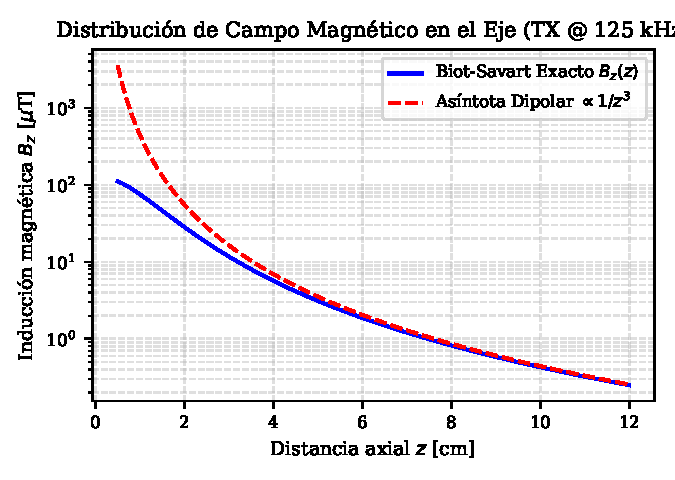
\includegraphics[width=0.92\columnwidth]{campo_b_distancia.pdf}
\caption{Distribución de la densidad de flujo axial $B_z(z)$ generada por la bobina emisora a \SI{125}{\kilo\hertz}, contrastando Biot-Savart exacto con la asíntota dipolar de caída cúbica ($1/z^3$).}
\label{fig:campo_b}
\end{figure}

La Fig.~\ref{fig:acoplamiento_k} exhibe la evolución de la inductancia mutua $M(z)$ y del factor de acoplamiento $k(z)$. A una distancia de \SI{1.0}{\centi\meter}, el acoplamiento es $k \approx 0.08$, cayendo a $k \approx \num{0.79e-3}$ a \SI{7.0}{\centi\meter}.

\begin{figure}[htbp]
\centering
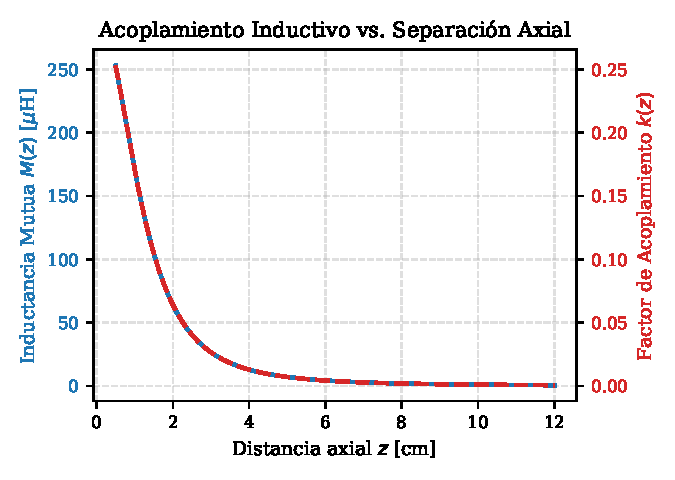
\includegraphics[width=0.92\columnwidth]{acoplamiento_k_distancia.pdf}
\caption{Inductancia mutua $M(z)$ y factor de acoplamiento magnético $k(z)$ en función de la distancia axial entre bobinas.}
\label{fig:acoplamiento_k}
\end{figure}

La simulación en el dominio de la frecuencia en SPICE (Fig.~\ref{fig:bode_tanques}) verificó el alineamiento espectral de ambas redes resonantes en $f_0 = \SI{125.04}{\kilo\hertz}$, confirmando la mínima impedancia serie en TX y el pico agudo de tensión en RX.

\begin{figure}[htbp]
\centering
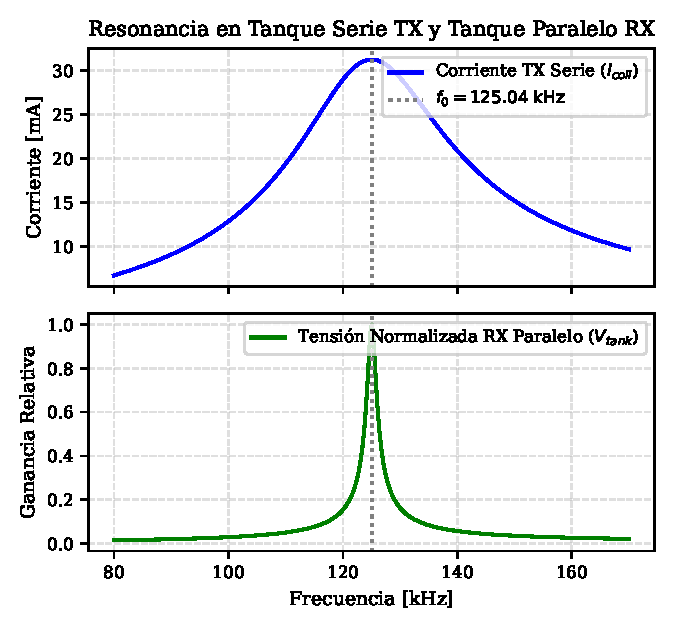
\includegraphics[width=0.92\columnwidth]{respuesta_frecuencia_tanques.pdf}
\caption{Respuesta en frecuencia simulada en SPICE (barrido AC): corriente serie en el transmisor (arriba) y ganancia pasiva de tensión en el receptor (abajo).}
\label{fig:bode_tanques}
\end{figure}

\subsection{Formas de Onda y Oscilogramas Experimentales}
\label{subsec:oscilogramas}

El prototipo se montó sobre la bancada de pruebas (Fig.~\ref{fig:montaje_experimental}) transmitiendo tramas continuas a \SI{250}{\text{bps}}.

\begin{figure}[htbp]
\centering
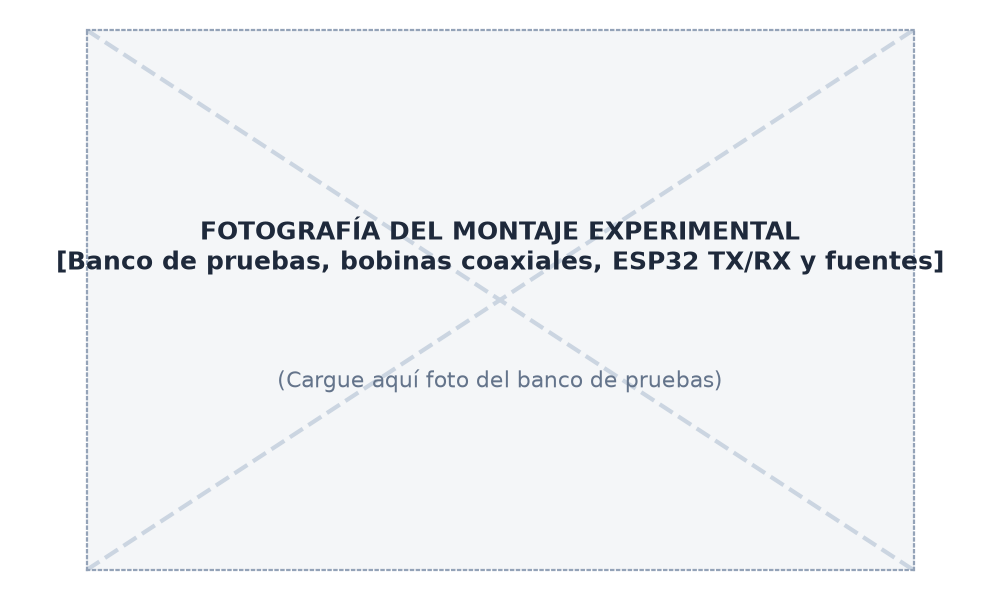
\includegraphics[width=0.88\columnwidth]{placeholder_montaje.png}
\caption{Banco de pruebas experimental: soporte milimétrico en PLA, bobinas RFID coaxiales sintonizadas y circuitos TX/RX con microcontroladores ESP32.}
\label{fig:montaje_experimental}
\end{figure}

En la Fig.~\ref{fig:osc_tx} se observa la concordancia temporal entre la señal de modulación binaria generada por el pin \texttt{GPIO18} del ESP32 y las ráfagas senoidales de \SI{125}{\kilo\hertz} en la bobina emisora.

\begin{figure}[htbp]
\centering
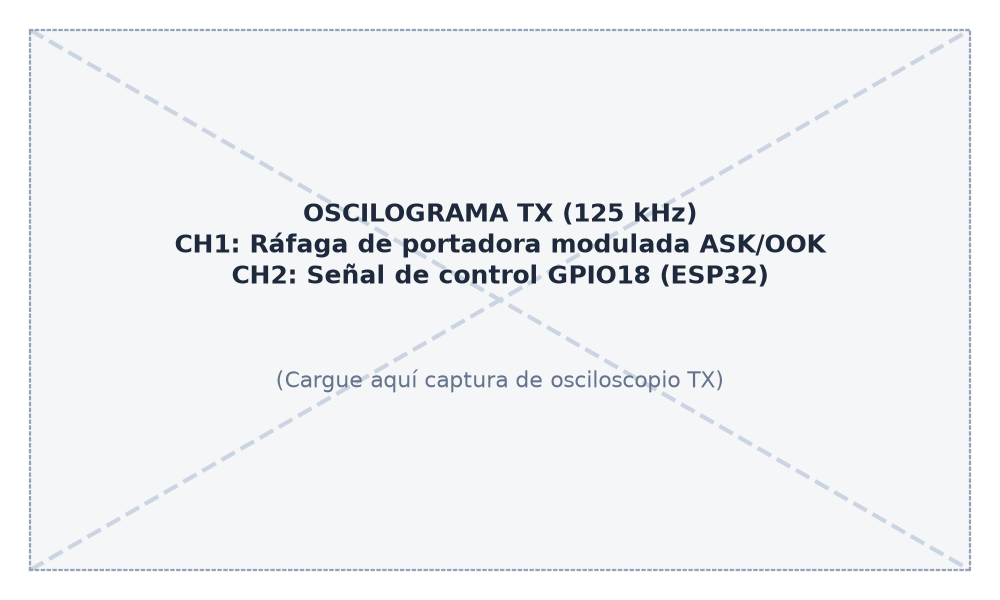
\includegraphics[width=0.88\columnwidth]{placeholder_osc_tx.png}
\caption{Oscilograma en el transmisor: moduladora digital OOK en \texttt{GPIO18} (arriba) y portadora de \SI{125}{\kilo\hertz} entregada a la bobina serie (abajo).}
\label{fig:osc_tx}
\end{figure}

La Fig.~\ref{fig:osc_rx_amp} ilustra la tensión de milivoltios captada en el tanque receptor y la señal preamplificada a la salida del MCP6002, conservando linealidad sin recorte rail-to-rail.

\begin{figure}[htbp]
\centering
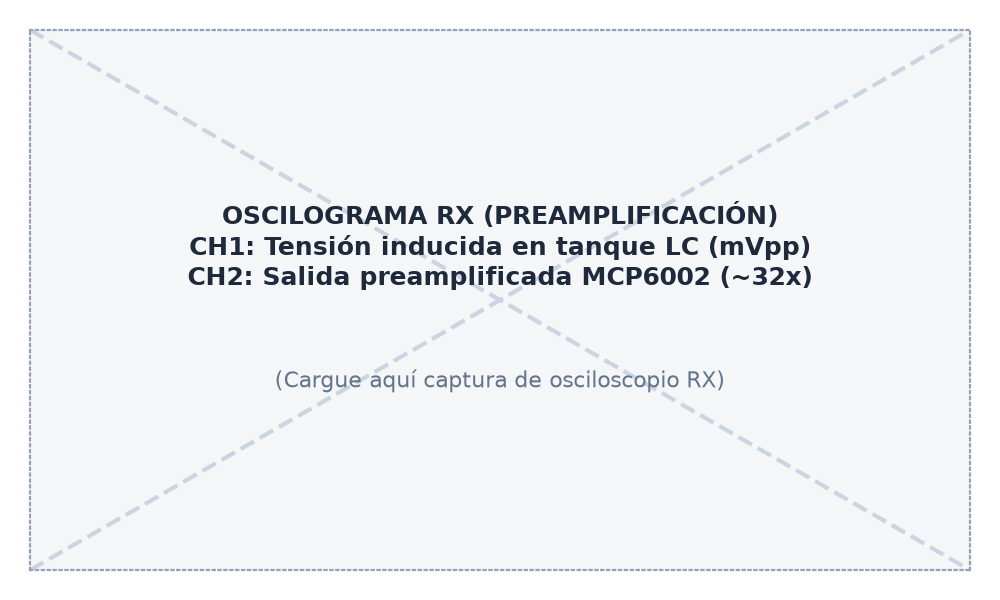
\includegraphics[width=0.88\columnwidth]{placeholder_osc_rx_amp.png}
\caption{Oscilograma en recepción: señal débil en el tanque LC paralelo (arriba) y señal amplificada a la salida del MCP6002 (abajo).}
\label{fig:osc_rx_amp}
\end{figure}

Por último, en la Fig.~\ref{fig:osc_demod} se evidencia la envolvente filtrada tras el diodo BAT85 y la conmutación nítida del comparador LM393, entregando un tren de datos digital de \SI{0}{\volt} a \SI{3.3}{\volt} libre de oscilaciones parásitas.

\begin{figure}[htbp]
\centering
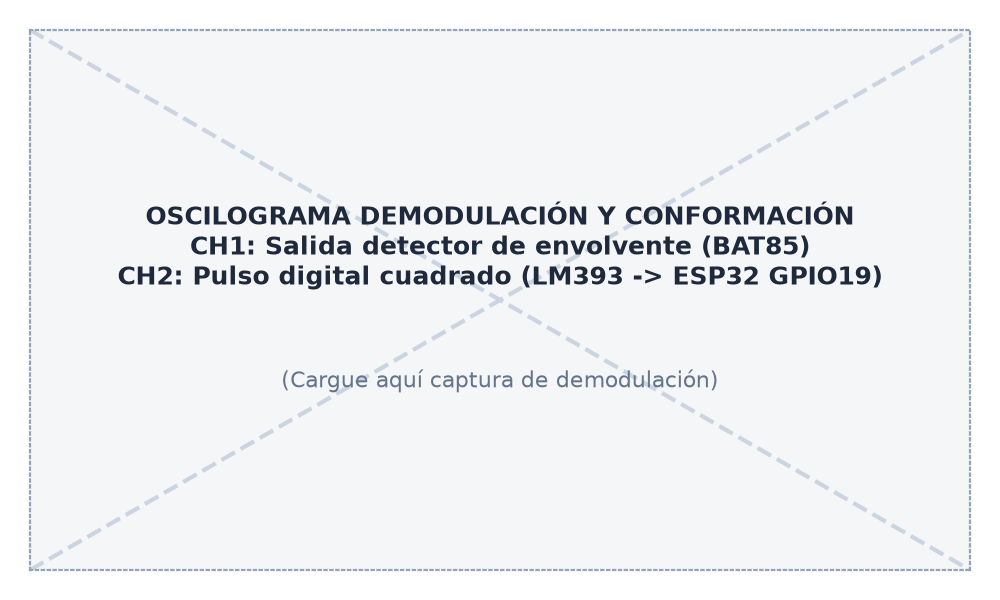
\includegraphics[width=0.88\columnwidth]{placeholder_osc_demod.png}
\caption{Demodulación y conformación: envolvente filtrada a la salida del diodo BAT85 (arriba) y pulsos digitales conformados hacia el ESP32 (abajo).}
\label{fig:osc_demod}
\end{figure}

\subsection{Mediciones Experimentales vs. Modelo y Verificación Digital}
\label{subsec:mediciones_experimentales}

Se efectuaron barridos sistemáticos de distancia axial entre \SI{1.0}{\centi\meter} y \SI{10.0}{\centi\meter}. En cada distancia se enviaron 100 tramas consecutivas con carga útil de 8 bytes, validando su recepción mediante el checksum CRC-8.

\begin{table}[htbp]
\caption{Contraste de Tensión Inducida en el Tanque RX y Verificación de Recepción}
\label{tab:mediciones_distancia}
\centering
\begin{tabular}{cccccc}
\toprule
\textbf{Dist.} & \textbf{$M_{\text{teor}}$} & \textbf{$V_{\text{tank}}$ Teór.} & \textbf{$V_{\text{tank}}$ Sim.} & \textbf{$V_{\text{tank}}$ Med.} & \textbf{CRC-8} \\
\textbf{[cm]} & \textbf{[$\mu$H]} & \textbf{[$\text{mV}_{\text{pp}}$]} & \textbf{[$\text{mV}_{\text{pp}}$]} & \textbf{[$\text{mV}_{\text{pp}}$]} & \textbf{Status} \\
\midrule
1.0 & 79.48 & 3912.4 & 3325.5 & 3051.7 & Válido \\
2.0 & 26.69 & 1313.8 & 1116.7 & 1024.7 & Válido \\
3.0 & 9.42  & 463.7  & 394.1  & 361.7  & Válido \\
4.0 & 4.14  & 203.8  & 173.2  & 158.9  & Válido \\
5.0 & 2.15  & 105.8  & 89.9   & 82.5   & Válido \\
6.0 & 1.25  & 61.5   & 52.3   & 47.9   & Válido \\
7.0 & 0.79  & 38.8   & 33.0   & 30.2   & Válido \\
8.0 & 0.53  & 26.0   & 22.1   & 20.3   & Fallo \\
10.0& 0.27  & 13.3   & 11.3   & 10.4   & Fallo \\
\bottomrule
\end{tabular}
\end{table}

Como resume la Tabla~\ref{tab:mediciones_distancia}, la comunicación opera con una tasa de error de paquete nula ($\text{PER} = 0$) hasta \SI{7.0}{\centi\meter}. A \SI{8.0}{\centi\meter}, la tensión inducida de \SI{20.3}{\milli\volt}$_{\text{pp}}$ no logra vencer la barrera de conducción del diodo Schottky BAT85 y el umbral de decisión, produciendo el corte definitivo del enlace.

En los ensayos de orientación angular a $z = \SI{4.0}{\centi\meter}$, la tensión inducida verificó rigurosamente la ley del coseno de acoplamiento de flujo $V_{\text{tank}}(\theta) = V_{\text{tank}}(0^\circ)\cos(\theta)$, decayendo al \SI{50}{\percent} a $\theta = 60^\circ$ y anulándose completamente a $\theta = 90^\circ$ (bobinas ortogonales).
